\documentclass[11pt,compress,t,notes=noshow, aspectratio=169, xcolor=table, usenames,dvipsnames]{beamer}

\usepackage{../../style/lmu-lecture}
% Defines macros and environments
% This file is included in slides and exercises

% Rarely used fontstyle for R packages, used only in 
% - forests/slides-forests-benchmark.tex
% - exercises/single-exercises/methods_l_1.Rnw
% - slides/cart/attic/slides_extra_trees.Rnw
\newcommand{\pkg}[1]{{\fontseries{b}\selectfont #1}}

% Spacing helpers, used often (mostly in exercises for \dlz)
\newcommand{\lz}{\vspace{0.5cm}} % vertical space (used often in slides)
\newcommand{\dlz}{\vspace{1cm}}  % double vertical space (used often in exercises, never in slides)
\newcommand{\oneliner}[1] % Oneliner for important statements, used e.g. in iml, algods
{\begin{block}{}\begin{center}\begin{Large}#1\end{Large}\end{center}\end{block}}

% Don't know if this is used or needed, remove?
% textcolor that works in mathmode
% https://tex.stackexchange.com/a/261480
% Used e.g. in forests/slides-forests-bagging.tex
% [...] \textcolor{blue}{\tfrac{1}{M}\sum^M_{m} [...]
% \makeatletter
% \renewcommand*{\@textcolor}[3]{%
%   \protect\leavevmode
%   \begingroup
%     \color#1{#2}#3%
%   \endgroup
% }
% \makeatother


\title{Interpretable Machine Learning}
% \author{LMU}
%\institute{\href{https://compstat-lmu.github.io/lecture_iml/}{compstat-lmu.github.io/lecture\_iml}}
\date{}

\begin{document}


% Set style/preamble.Rnw as parent.

% Load all R packages and set up knitr

% This file loads R packages, configures knitr options and sets preamble.Rnw as
% parent file
% IF YOU MODIFY THIS, PLZ ALSO MODIFY setup.Rmd ACCORDINGLY...

% Defines macros and environments

 \newcommand{\titlefigure}{figure/counterfactuals_obj}
\newcommand{\learninggoals}{
\item Understand the motivation behind CEs
\item Know why and how CEs are used
\item Recognize the philosophical foundations of counterfactual reasoning}

\lecturechapter{Counterfactual Explanations (CEs): Motivation}
\lecture{Interpretable Machine Learning}

% ------------------------------------------------------------------------------

\begin{frame}{Motivating Example: Credit Risk \& CE}
        %\begin{center}
            $\textbf{x}$: customer and credit information \hfill $y$: grant or reject credit \
        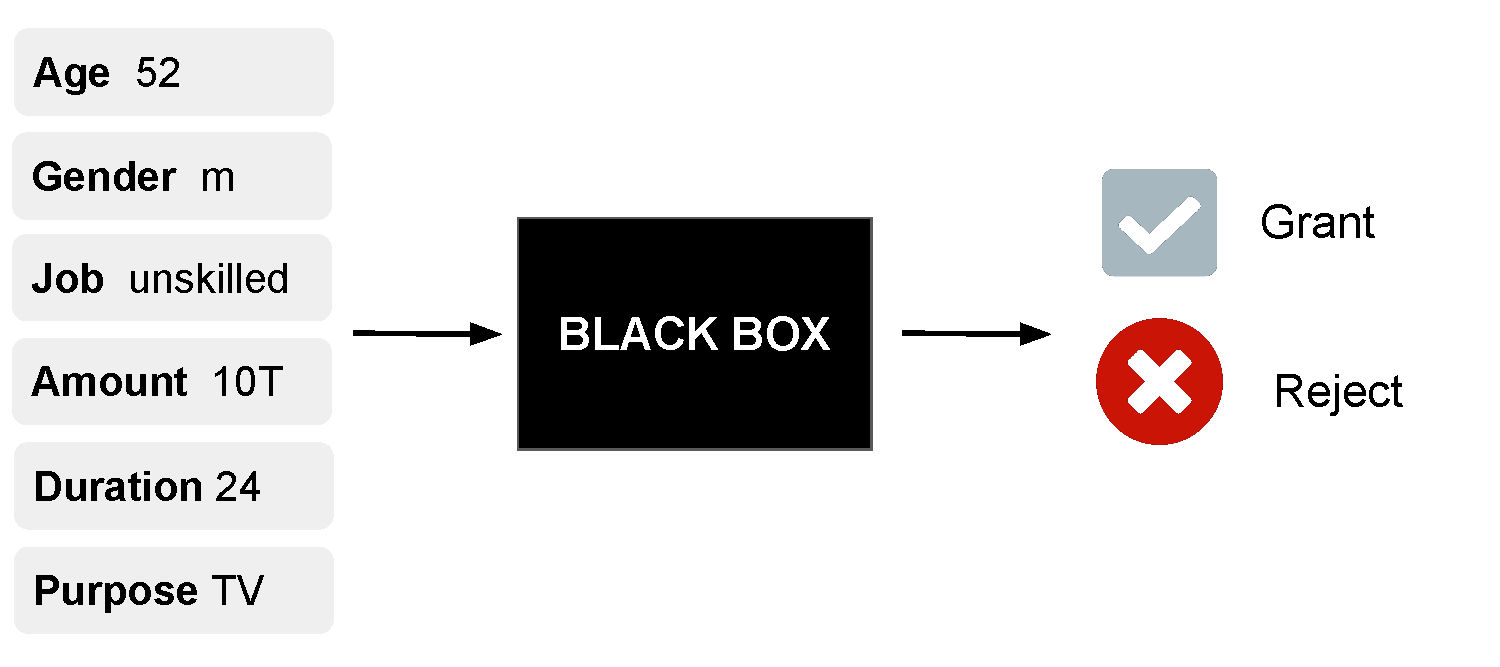
\includegraphics[width=\linewidth, page=1]{figure/counterfactuals_credit.pdf} 
        %\end{center}

	Potential questions:
	\begin{itemize}
		\item Why was the credit rejected?
		\item Is this decision fair compared with similar applicants?
		\item \textbf{How should $\xv$ be changed so that the credit is accepted?}
	\end{itemize}
\end{frame}


\begin{frame}{Motivating Example: Credit Risk \& CE}
	Counterfactual Explanations provide answers in the form of "What-If"-scenarios.
	
    \includegraphics[width=\linewidth, page=2]{figure/counterfactuals_credit.pdf}

	``If the applicant had higher skills and the credit amount had been reduced to \$8.000,\\ the loan would have been granted."  \\[0.2cm]

\end{frame}


% \begin{frame}{Counterfactual Explanations: Main Idea}
% 	\begin{itemize}[<+->]
% 	    \item Counterfactual explanations == counterfactuals == CEs
% 	    \item Explain particular predictions of an ML model by presenting an alternative input whose prediction equals a desired outcome
% 		\item Represent \textbf{close neighbors} of a data point we are interested in,\\ but belonging to the \textbf{desired outcome}
% 		\item Show which minimal changes in input suffice to receive a different outcome\\
% 		$\leadsto$ Useful if changing input features is possible (e.g., by changing behaviour)
% 		\item The targeted audience of CEs are often end-users%, not ML engineers
% 	\end{itemize}
% \end{frame}


\begin{frame}{Core Definition and Purpose of CE}
  \begin{itemize}
    \item<1-> \textbf{Counterfactual explanation (CE):} Hypothetical input \(\mathbf{x}'\) close to the data point of interest $\mathbf{x}$ whose prediction equals a user-defined desired outcome \(y'\)
    \item<2-> \textbf{Proximity constraint:} %Find \(\mathbf{x}' \approx \mathbf{x}\) such that
      \[
      \text{Find} \quad \mathbf{x}' \approx \mathbf{x} \quad\text{such that} \quad f(\mathbf{x}') = y' \quad\text{and distance}\quad 
        d(\mathbf{x},\mathbf{x}') \quad \text{is minimal}
      \]
    \item<3-> \textbf{Minimal actionable changes:} Difference \(\mathbf{x}'-\mathbf{x}\) shows the smallest feature change a user could realize in practice
    \item<4-> \textbf{Primary audience:} 
    \begin{itemize}
        \item Individuals aiming to alter model predictions 
        \item ML engineers exploring model behavior under adversarial conditions\\
        $\leadsto$ how small text changes in email flip  prediction from "spam" to "no spam"
    \end{itemize}
  \end{itemize}
\end{frame}


\begin{frame}{Interpretive Aims \& Roles}
	CEs can serve various purposes; the user can decide what to learn from them, e.g.:  \\[0.2cm]
	``If the person had been \textbf{one year older} and the \textbf{credit amount had been increased} to \$12.000, the credit would have been granted."  \\[0.2cm]
	\pause
	\begin{itemize}[<+->]
		\itemsep1.2em
		\item \textbf{Guidance for future actions:}\\ \textit{Ok, I will apply again next year for the higher amount.}
		\item \textbf{Provide reasons:}\\ \textit{Interesting, I did not know that age plays a role in loan applications.}
		\item \textbf{Provide grounds to contest the decision:}\\ \textit{How dare you, I do not want to be discriminated for my age in an application.}
		\item \textbf{Detect model biases:}\\ \textit{There is a bug, an increase in amount should not increase approval rates.}
	\end{itemize}
\end{frame}


%------------------------------------------------------------
\begin{frame}{Philosophical Foundations \citebutton{Lewis (1973)}{https://doi.org/10.2307/2273738}}

Counterfactuals have a long tradition in analytic philosophy\\
$\leadsto$ A \textbf{counterfactual conditional} takes the form:

\begin{center}
  \emph{"If $S$ had occurred, $Q$ would have occurred."}
\end{center}

  \begin{itemize}%[<+->]
    \item $S$: past event that never happened 
    $\leadsto$ CE run contrary to fact
    \item Statement is true iff $Q$ holds in all \textbf{closest} worlds where $S$ is true
    \item Closest worlds preserve laws and change as few facts as possible (related to $S$)
    %\item \alert{Debate}: what counts as "closest" is controversial in philosophy
  \end{itemize}
\end{frame}

%------------------------------------------------------------
\begin{frame}{Philosophical Foundations}
  \begin{itemize}%[<+->]
    \item<1-> CEs have largely been studied to explain causal dependence
    \item<1-> \textbf{Causal dependence}: $Q$ depends on $S$   $\Leftrightarrow$ without $S$, no $Q$\\
    $\leadsto$ Good CEs point to critical causal factors that drove the algorithmic decision\\
    $\leadsto$ \textbf{CE objective}: find $\mathbf{x}' \!\approx\! \mathbf{x}$ with $f(\mathbf{x}')=y'$ to expose causal features
    \item<2-> Relaxing closeness may add causally irrelevant edits to the explanation\\
$\leadsto$ e.g., suggest to lower loan \emph{and} increase age (but only loan matters)

\item<3-> CEs are contrastive: Explain a decision by comparing it to a different outcome\\
$\leadsto$ If age were 30 instead of 60, loan would have been \$9k instead of rejected\\%\$40k\\
$\leadsto$ Answers contrastive question: ``Why Q' instead of Q?'' (preferred by humans)

    % \item \textbf{Alternative view}: Pearl (2009) models causality via graphs, then derives counterfactuals from the graph
  \end{itemize}
\end{frame}















% \begin{frame}{Philosophical Basis}
% %Interestingly, counterfactuals have a long-standing tradition in philosophy and, in fact the IML discussion of CEs is based on the work of Lewis (1973).
% Counterfactuals have a long-standing tradition in analytic philosophy\\
% $\leadsto$ %and, in fact the IML discussion of CEs is based on the work of Lewis (1973).
% Accoding to \citebutton{Lewis (1973)}{https://doi.org/10.2307/2273738}, a \textbf{counterfactual conditional} is a statement of  form:

% \begin{center}
% ``If $S$ was the case, $Q$ would have been the case."
% 		%\label{eq:sent}
% \end{center}

% \pause

% 	\begin{itemize}[<+->]
% 		\item $S$ is an event that must relate to a past event that didn't occur\\ $\leadsto$ counterfactuals run \textbf{contrary} to the \textbf{facts}
% 		\item Above statement is true, if in all possible worlds most similar to the actual world where $S$ had been the case, $Q$ would have been the case
% 		\item A world is similar to another if laws are maximally preserved between the worlds and only a few facts are changed
% %		\item Lewis's proposal is hotly debated in philosophy, particularly his notion of similarity between worlds remains controversial.
% 	\end{itemize}
% \end{frame}

% \begin{frame}{Philosophical Basis}
% % According to Lewis:\newline
% %``$Q$ causally depends on $S$ iff, if $S$ were not the case $Q$ would not have been the case.''
% 	\begin{itemize}%[<+->]
% 	\item Counterfactuals have largely been studied to explain causal dependence
% 		\item Causal dependence underlies the explanatory power\\
% 		$\leadsto$ good CEs point to critical causal factors that drove the algorithmic decision
% 		\item If maximal closeness is relaxed, causally irrelevant factors can become part of the explanation\\
% 		$\leadsto$ e.g., decreasing loan amount by \$20.000 and being one year older is recommended by the explainer although only loan amount might be causally relevant
% 		%Think of a case when a decrease in amount by \$20.000 and being one year older is recommended by the explainer to receive the loan while changing only the former suffices
% 		\item CEs are often contrastive, i.e., they explain a decision by referring to an alternative outcome\\
% 		$\leadsto$ e.g., if the loan applicant was 30 instead of 60 years old, the approved loan would have been over \$100.000 instead of \$40.000%This is also the reason why counterfactuals must be maximally close to initial inputs, otherwise changes are only sufficient but some of them might be unnecessary.
% %		\item Current research on causality is based on Pearl's (2009) causal graphs. Instead of defining causality in terms of counterfactuals, Pearl's approach turns the story around and necessitates a representation of causal mechanisms to define CEs.
% 	\end{itemize}
% %\footnote[frame]{Lewis, David (1973). Counterfactuals. Cambridge, MA: Harvard University Press. ISBN 9780631224952. }
% \end{frame}

%\begin{frame}{Philosophical Basis: CEs as Contrastive}
%CEs are or can be easily translated into contrastive explanations and often vice versa. Contrastive explanations are answers to a question of the form ``why did Q' occur instead of Q?''.
%	\begin{itemize}
%	    \item  Contrastive explanations answer these questions by \textbf{contrasting} the actual scenario with a different scenario $S$ in which $Q$ had occurred.
%		\item According to psychologists [Miller (2019)], contrastive explanations are the gold standard of explanations in human-to-human interaction.
%		\item A CE becomes contrastive if its antecedent $S$ is presented in contrast to the actual scenario.
%	\end{itemize}
%\end{frame}


\endlecture
\end{document}
